        	\begin{question}{31}{Trigonométrie}{1}{/}
				Quel est le sinus de $0$?
            \end{question}
            \begin{reponses}
            	\item[false] $\frac{\sqrt{2}}{2}$
            	\item[false] 1
                \item[false] $1/2$
                \item[true] 0
            \end{reponses}
			%%%%%%%%%%%%%%%%%%%%%%%%%%%%%%%%%%%%%
            \begin{question}{31}{Trigonométrie}{2}{/}
                Que vaut le cosinus de l'angle représenté ci-dessous?
                \begin{center}
                	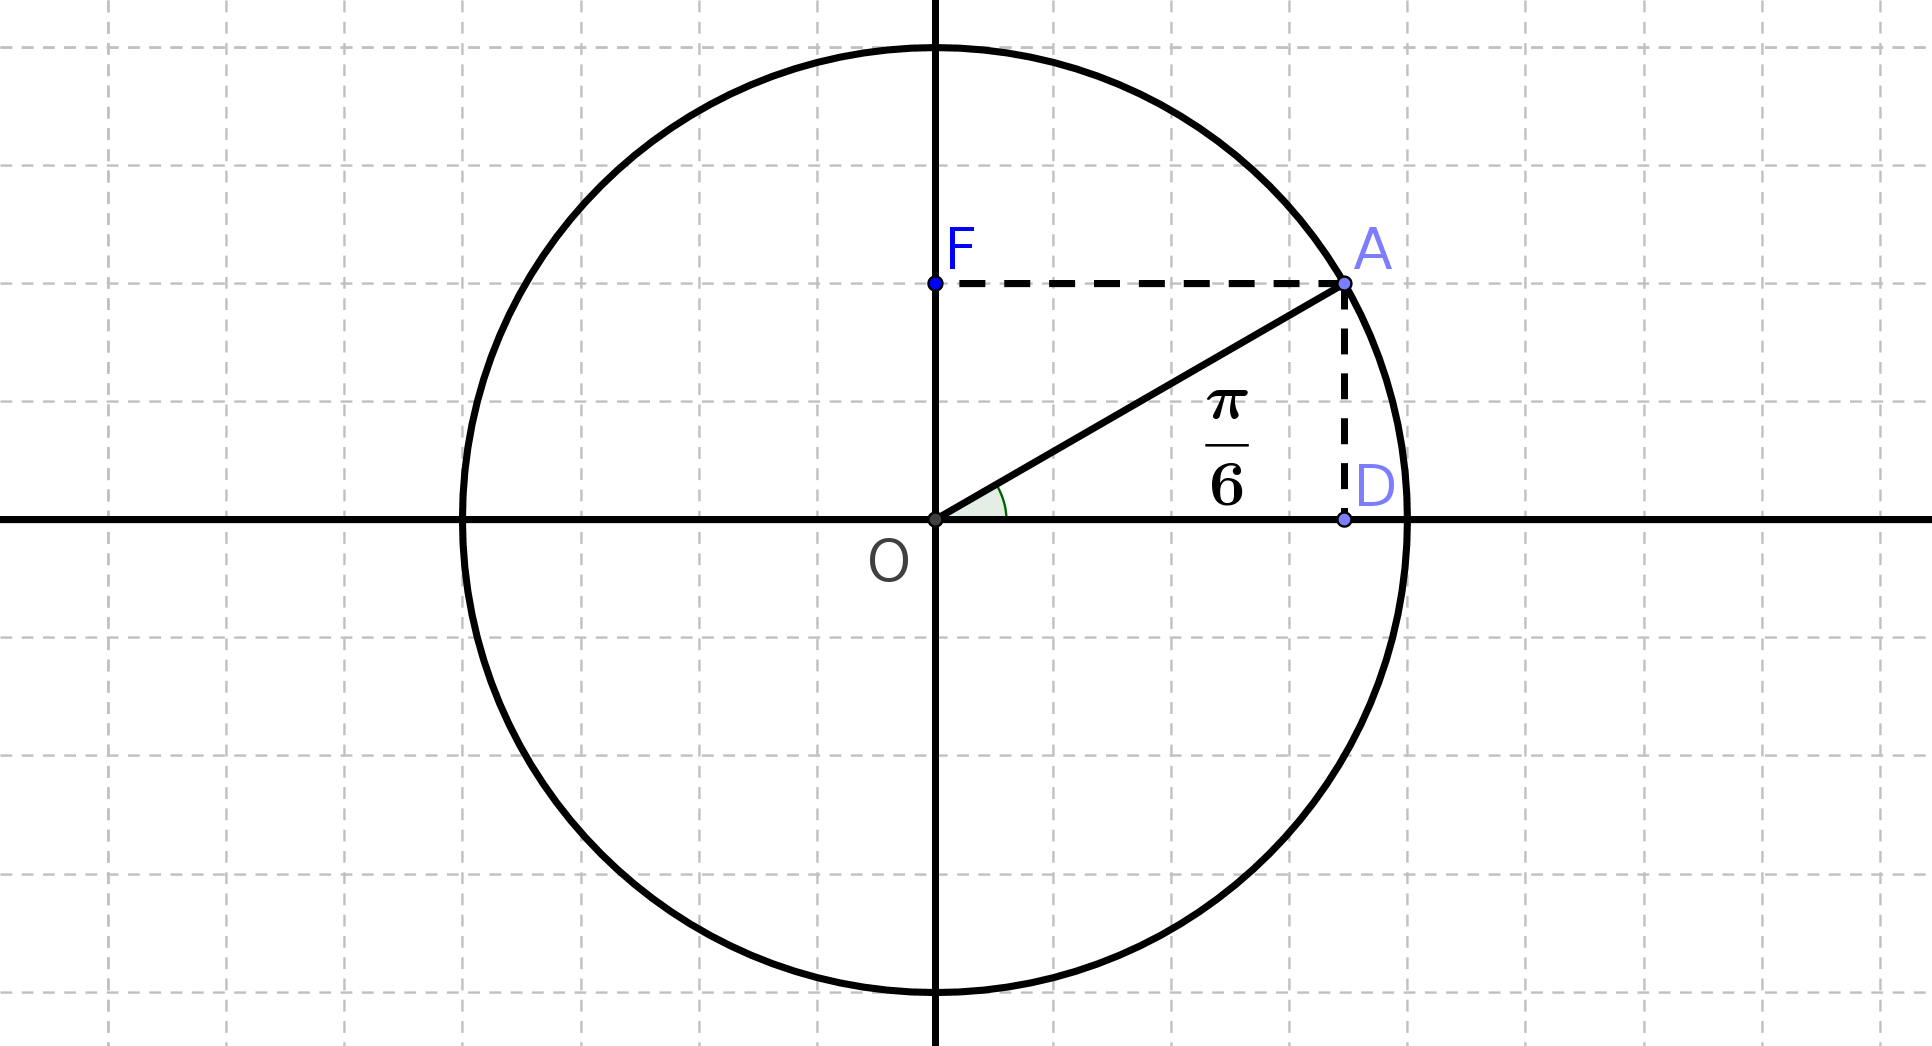
\includegraphics[width=0.5\textwidth]{Philippe/Figures_Philippe/trigo_1_3.png}
                \end{center}
            \end{question}
            \begin{reponses}
                \item[false] $\frac{\sqrt{2}}{2}$
                \item[false] $-\frac{\sqrt{2}}{2}$
                \item[false] $\frac{1}{2}$
                \item[true] $\frac{\sqrt{3}}{2}$
            \end{reponses}
            %%%%%%%%%%%%%%%%%%%%%%%%%%%%%%%%%%%%%
            \begin{question}{31}{Trigonométrie}{2}{/}
				Parmi les angles ci-dessous, lequel a pour cosinus $\frac{\sqrt{3}}{2}$?
            \end{question}
            \begin{reponses}
            	\item[false] $\frac{\pi}{3}$
            	\item[true] $\frac{\pi}{6}$
                \item[false] $\frac{\pi}{4}$
                \item[false] $\pi$
            \end{reponses}
            %%%%%%%%%%%%%%%%%%%%%%%%%%%%%%%%%%%%%
            \begin{question}{31}{Trigonométrie}{2}{/}
            	Quel est le sinus de $\frac{\pi}{6}$? 
            \end{question}
            \begin{reponses}
                \item[true] $1/2$
                \item[false] $-1/2$
                \item[false] 1
                \item[false] -1
            \end{reponses}
            %%%%%%%%%%%%%%%%%%%%%%%%%%%%%%%%%%%%%
        	\begin{question}{31}{Trigonométrie}{3}{/}
				L'aiguille des heures forme un certain angle avec l'horizontal (0 quand il est 3 heures, $+\frac{\pi}{2}$ quand il est midi). Quel est le cosinus de l'angle ainsi formé quand il est 1 heure? 
            \end{question}
            \begin{reponses}
            	\item[false] $\frac{\sqrt{3}}{2}$
            	\item[false] $-1/2$
                \item[false] $\frac{\sqrt{2}}{2}$
                \item[true] $1/2$
            \end{reponses}
			%%%%%%%%%%%%%%%%%%%%%%%%%%%%%%%%%%%%%
        	\begin{question}{31}{Trigonométrie}{3}{/}
				La vitesse d'un objet fait un angle de $-\frac{\pi}{4}$ avec l'axe des $x$. Quel est le sinus de cet angle?
            \end{question}
            \begin{reponses}
            	\item[false] $\frac{\sqrt{3}}{2}$
            	\item[false] $\frac{\sqrt{2}}{2}$
                \item[false] $-\frac{\sqrt{3}}{2}$
                \item[true] $-\frac{\sqrt{2}}{2}$
            \end{reponses}
			%%%%%%%%%%%%%%%%%%%%%%%%%%%%%%%%%%%%%
